\chapter{Simulations} 

Cette annexe a pour but de tester l'impact de la distribution des inflorescences en entrée d'une version du modèle donnée sur le nombre de larves total prédit trouvés par celle-ci.

Pour faire cela, on se donne deux dynamiques d'inflorescences différentes : l'une ne possède qu'un seul \textit{flush}, l'autre en possède deux (voir figure~\ref{fig:flush}). 
Il est important de noter que le nombre d'inflorescences considérées sera identique pour les deux dynamiques, sans quoi comparer le nombre de larves ne serait pas pertinent.

\begin{figure}[h]
 \centering
 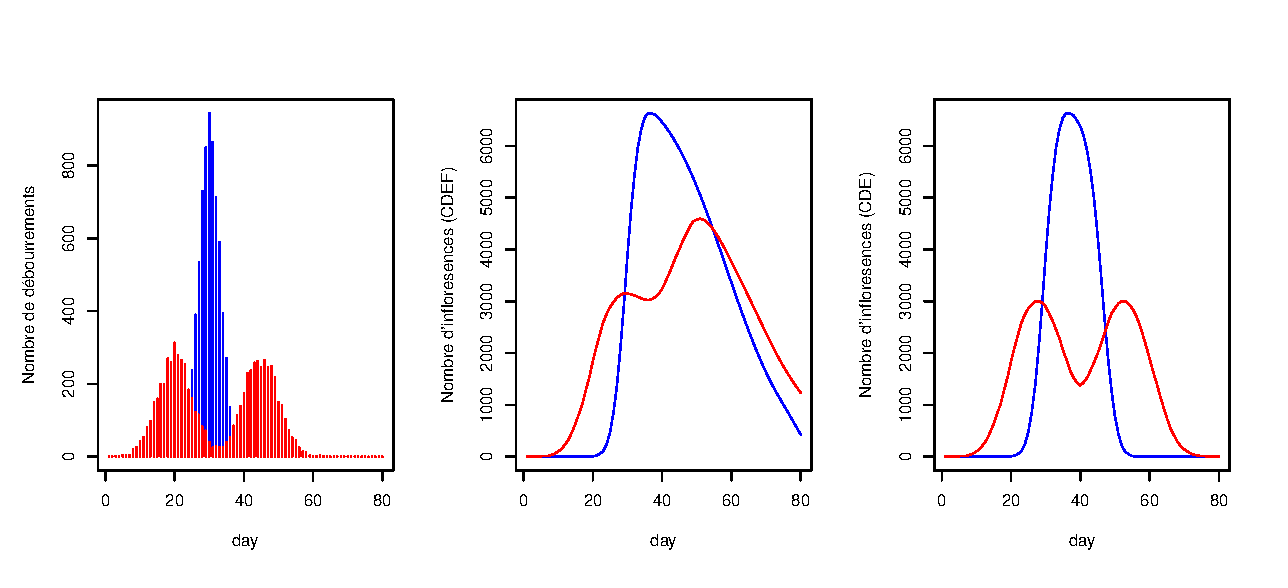
\epsfig{file = plots/dynamiques.eps, scale = 0.7}
 \caption{Représentation des dynamiques d'inflorescences simulées vivantes (au milieu) ou aux stades phénologiques C, D et E (à droite) avec les débourrements correspondants (à gauche). }
 \label{fig:flush}
\end{figure}

Pour être raccord avec ce qui a été fait précédemment, on utilisera les inflorescences vivantes (aux stades C, D, E et F) dès lors que l'on utilisera le modèle A, et les inflorescences aux stades phénologiques C, D et E lorsque l'on utilisera les modèles C ou D.

\section{Modèle A}

On s'intéresse aux résultats obtenus en utilisant les jeux de paramètres correspondant aux deux premières solutions--types trouvées (la troisième ne nous semble pas pertinente).
Les résultats pour la première solution--type sont :
{%
\newcommand{\mc}[3]{\multicolumn{#1}{#2}{#3}}
\begin{center}
\begin{tabular}{lllllll}
\mc{7}{c}{\textbf{Paramètres}}\\
$\gamma$ & $p_{\text{m}}$ & $\mu_{\text{ER}}$ & $\mu_{\text{EH}}$ & $k$ & \texttt{stock} & $E_0\mu_{\ell}$\\
0.08 & 0.494 & 0.976 & 0.046 & 1.928 & 5600 & 3.084\\\hline
\mc{2}{r}{ } & \mc{5}{r}{Nombre de larves total}\\
\mc{2}{r}{1 flush} & \mc{5}{r}{216 204}\\
\mc{2}{r}{2 flushs} & \mc{5}{r}{206 048}
\end{tabular}
\end{center}
}%
Les résultats pour la deuxième solution--type sont :
{%
\newcommand{\mc}[3]{\multicolumn{#1}{#2}{#3}}
\begin{center}
\begin{tabular}{lllllll}
\mc{7}{c}{\textbf{Paramètres}}\\
$\gamma$ & $p_{\text{m}}$ & $\mu_{\text{ER}}$ & $\mu_{\text{EH}}$ & $k$ & \texttt{stock} & $E_0\mu_{\ell}$\\
0.000 & 0.968 & 1.000 & 0.025 & 0.100 & 14483 & 6.260\\\hline
\mc{2}{r}{ } & \mc{5}{r}{Nombre de larves total}\\
\mc{2}{r}{1 flush} & \mc{5}{r}{37 079}\\
\mc{2}{r}{2 flushs} & \mc{5}{r}{100 018}
\end{tabular}
\end{center}
}%

Au vu des deux résultats, il est difficile de proposer une interprétation tant aucune tendance ne semble se dégager lorsqu'on l'on change de jeu de paramètres.

\section{Modèle C}

On réitère en utilisant le modèle C qui semblait obtenir des résultats plus pertinent.
Les résultats pour la première solution--type sont :
{%
\newcommand{\mc}[3]{\multicolumn{#1}{#2}{#3}}
\begin{center}
\begin{tabular}{lllllll}
\mc{7}{c}{\textbf{Paramètres}}\\
$\gamma$ & $p_{\text{m}}$ & $\mu_{\text{ER}}$ & $\mu_{\text{EH}}$ & $k$ & \texttt{stock} & $E_0\mu_{\ell}$\\
0.115 & 0.189 & 0.898 & 0.012 & 1.877 & 515 & 3.097\\\hline
\mc{2}{r}{ } & \mc{5}{r}{Nombre de larves total}\\
\mc{2}{r}{1 flush} & \mc{5}{r}{140 138}\\
\mc{2}{r}{2 flushs} & \mc{5}{r}{170 557}
\end{tabular}
\end{center}
}%

Les résultats pour la deuxième solution--type sont :
{%
\newcommand{\mc}[3]{\multicolumn{#1}{#2}{#3}}
\begin{center}
\begin{tabular}{lllllll}
\mc{7}{c}{\textbf{Paramètres}}\\
$\gamma$ & $p_{\text{m}}$ & $\mu_{\text{ER}}$ & $\mu_{\text{EH}}$ & $k$ & \texttt{stock} & $E_0\mu_{\ell}$\\
0.004 & 0.490 & 0.990 & 0.018 & 0.242 & 9970 & 5.638\\\hline
\mc{2}{r}{ } & \mc{5}{r}{Nombre de larves total}\\
\mc{2}{r}{1 flush} & \mc{5}{r}{29 764}\\
\mc{2}{r}{2 flushs} & \mc{5}{r}{122 692}
\end{tabular}
\end{center}
}%

Ici une tendance se dégage : il y a moins de larves lorsque la dynamique de floraison ne présente qu'un seul \textit{flush}.
On peut remarquer que la diminution est d'autant plus forte lorsque le modèle ne fait appel qu'à peu d'individus exogènes

\section{Modèle D}

On s'intéresse à présent au modèle D, qui comprend un phénomène de saisonnalité.
Les résultats pour la première solution--type sont :
{%
\newcommand{\mc}[3]{\multicolumn{#1}{#2}{#3}}
\begin{center}
\begin{tabular}{llllllll}
\mc{8}{c}{\textbf{Paramètres}}\\
$\gamma$ & $p_{\text{m}}$ & $\mu_{\text{ER}}$ & $\mu_{\text{EH}}$ & $k$ & \texttt{stock} & $E_0\mu_{\ell}$ & $\xi$\\
0.021 & 0.105 & 0.938 & 0.916 & 1.992 & 516 & 6.018 & 0.004\\\hline
\mc{2}{r}{ } & \mc{6}{r}{Nombre de larves total}\\
\mc{2}{r}{1 flush} & \mc{6}{r}{81 073}\\
\mc{2}{r}{2 flushs} & \mc{6}{r}{113 068}
\end{tabular}
\end{center}
}%

Les résultats pour la deuxième solution--type sont :
{%
\newcommand{\mc}[3]{\multicolumn{#1}{#2}{#3}}
\begin{center}
\begin{tabular}{llllllll}
\mc{8}{c}{\textbf{Paramètres}}\\
$\gamma$ & $p_{\text{m}}$ & $\mu_{\text{ER}}$ & $\mu_{\text{EH}}$ & $k$ & \texttt{stock} & $E_0\mu_{\ell}$ & $\xi$\\
0.019 & 0.131 & 0.999 & 0.743 & 0.262 & 508 & 6.190 & 0.060\\\hline
\mc{2}{r}{ } & \mc{6}{r}{Nombre de larves total}\\
\mc{2}{r}{1 flush} & \mc{6}{r}{63 686}\\
\mc{2}{r}{2 flushs} & \mc{6}{r}{104 882}
\end{tabular}
\end{center}
}%

La même tendance que pour le modèle C se dégage : une dynamique de floraison avec un unique \textit{flush} semble limiter la présence de larves.
